\documentclass[../opis-rozwiazania.tex]{subfiles}

\begin{document}

Opracowywany system składa się z następujących modułów:

\begin{itemize}
  \item nadzorcy,
  \item serwera wirtualizacji,
  \item aplikacji klienckiej,
  \item panelu administratora,
  \item brokera wiadomości,
  \item systemu katalogowego,
  \item dysku współdzielonego.
\end{itemize}

Schematyczny obraz systemu przedstawiony został na rysunku \ref{figure:architecture:system}.

\begin{figure}[h]
  \centering
  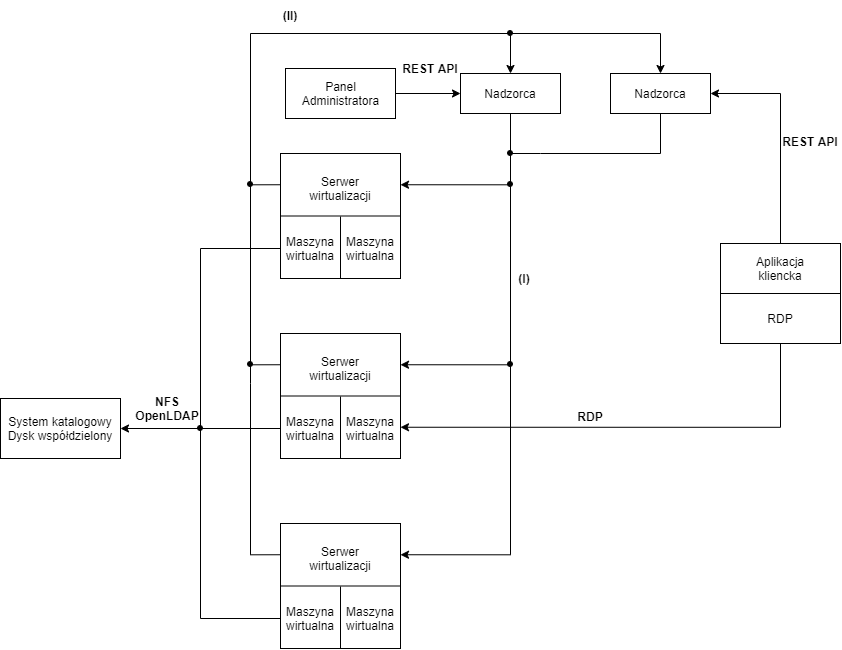
\includegraphics[width=\textwidth]{../diagrams/architecture.png}
  \caption{Schematyczna architektura systemu}
  \label{figure:architecture:system}
\end{figure}

Połączenia oznaczone liczbami rzymskimi oznaczają kolejki komunikacji za pośrednictwem brokera wiadomości, które opisane zostały w sekcji \ref{modules:broker}. Z założenia system powinien móc skalować się w dwóch wymiarach, to znaczy:
\begin{itemize}
  \item Zwiększanie liczby serwerów wirtualnych - zwiększenie liczby istniejących jednocześnie sesji.
  \item Zwiększenie liczby nadzorców - zwiększenie liczby obsługiwanych jednocześnie klientów oraz niezawodności systemu.
\end{itemize}

\subsection{Model systemu}

W celu zarządzania systemem, każdy z nadzorców musi posiadać dokładną wiedzę o jego aktualnym stanie. Informacje te przechowuje w strukturze nazywanej dalej modelem systemu. Ważne jest, że klasy modelu nie wykonują żadnych akcji poza modyfikacją przechowywanych danych. Wszelkie metody służą jedynie do zmiany stanu przechowywanego modelu w celu dopasowania go do rzeczywistego stanu, na podstawie otrzymanych danych. Przyczyną takiego stanu jest pierwsze z założeń komunikacji opisanych w sekcji \ref{communication:broker}. Sprawia ono, że zmiana modelu musi być następstwem pewnej akcji wykonanej przez serwer wirtualizacji. Schemat klas przedstawia rysunek \ref{figure:architecture:model}.

\begin{figure}[h]
  \centering
  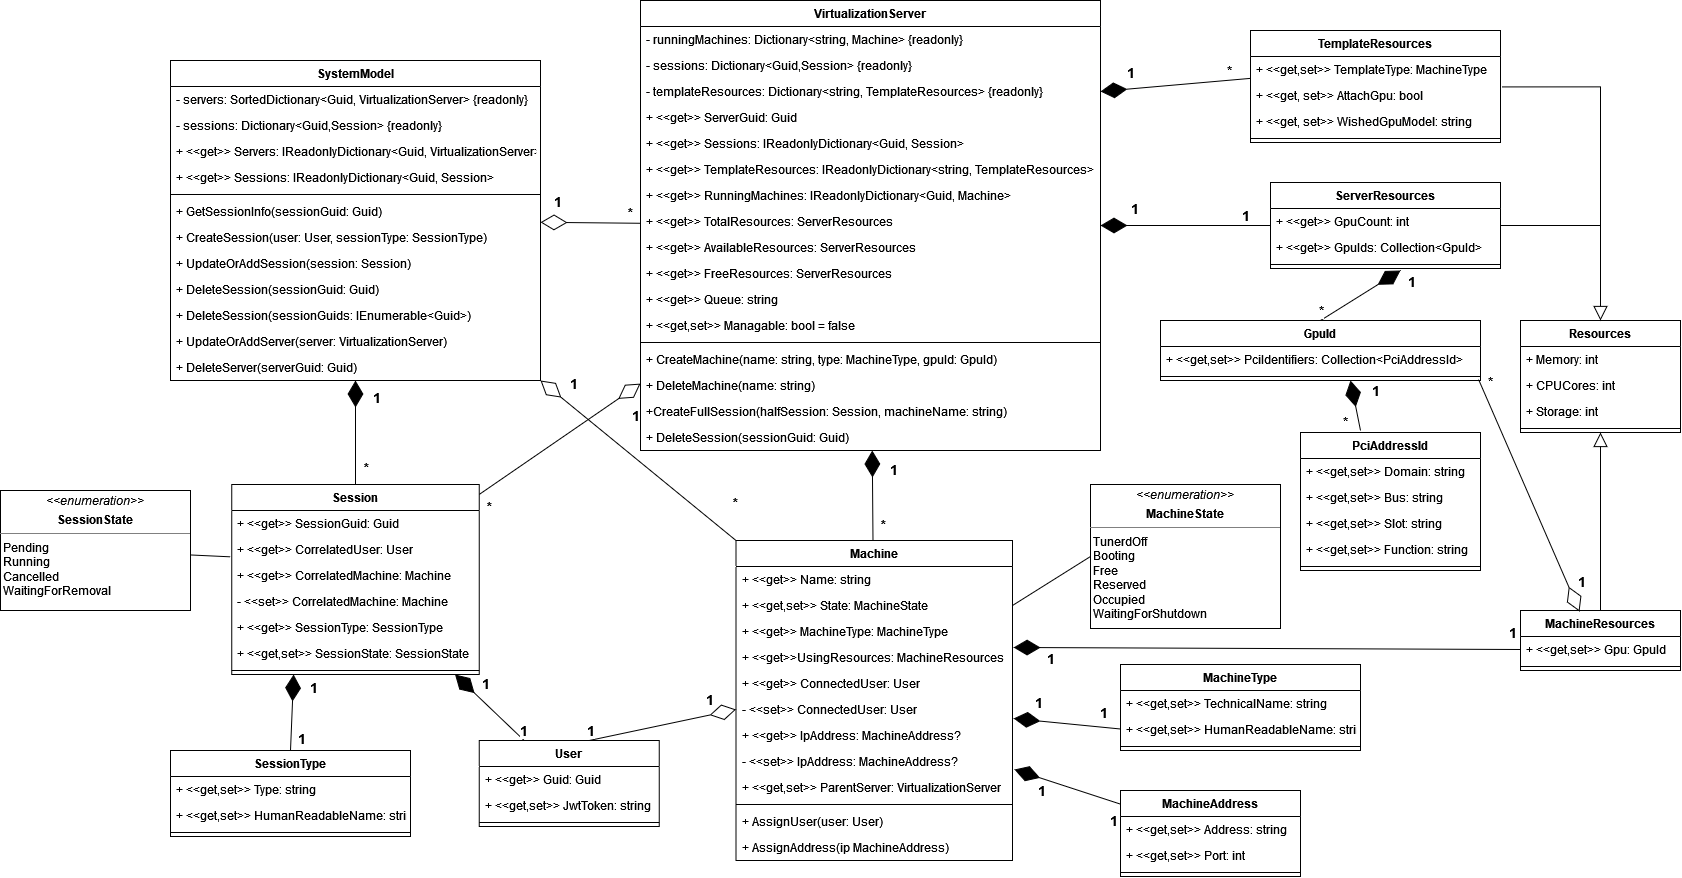
\includegraphics[width=\textwidth]{../diagrams/class_diagrams/system_model_v2.png}
  \caption{Schemat klas modelu systemu}
  \label{figure:architecture:model}
\end{figure}

Główną klasą modelu jest \texttt{SystemModel} zawierający informacje o aktualnie działających serwerach wirtualizacji oraz aktywnych sesjach. Klasa \texttt{VirtualizationServer} modeluje pojedynczy serwer wirtualizacji, jego zasoby, maszyny wirtualne oraz obsługiwane sesje. Przechowuje ona również informacje wymagane do komunikacji z daną instancją serwera.

Klasa \texttt{Resources} oraz jej pochodne opisują zasoby systemowe i są używane do przedstawienia zarówno zasobów maszyny jak i całego serwera wirtualizacji. Jej klasa pochodna \texttt{\seqsplit{TemplateResources}} służy do przechowywania informacji o zasobach potrzebnych do utworzenia maszyny danego typu.

\subsection{Nadzorca}
\label{modules:overseer}

Aplikacja mająca za zadanie obsługiwać komunikację z aplikacjami klienckimi oraz wysyłać polecenia do serwerów wirtualizacji. Udostępnia REST API (sekcja \ref{communication:api}), służące do komunikacji z aplikacjami klienckimi. Do komunikacji z serwerami wirtualizacji wykorzystuje kolejki wiadomości (sekcja \ref{modules:broker}).

Nadzorca przechowuje wewnętrznie model systemu zawierający informację o działających serwerach wirtualizacji i stanie ich maszyn. Na podstawie tego modelu moduł stwierdza, do której maszyny przypisać nowo utworzoną sesję. Wewnętrzne procesy skupione są wokół zmian modelu. Jeżeli proces wysłał do serwera wirtualizacji prośbę o zmianę stanu, to dalsze przetwarzanie odbywa się, gdy stan modelu został zaktualizowany, i na podstawie jego stanu podejmowane są decyzje.

Dzięki zastosowaniu kolejek wiadomości (sekcja \ref{modules:broker}) oraz zasad komunikacji (sekcja \ref{communication:broker}) w systemie może istnieć więcej niż jeden nadzorca. Instancje nadzorców działają niezależnie od siebie i przechowują identyczny model systemu. Dzięki temu uzyskujemy retencję i możemy zmniejszyć obciążenie poszczególnych nadzorców.

\subsection{Serwer wirtualizacji}
\label{modules:virtsrv}

Zadaniem serwera wirtualizacji jest uruchamianie i zarządzanie maszynami wirtualnymi, z którymi łączy się użytkownik systemu. Komunikuje się on z nadzorcami i wykonuje operacje na maszynach wirtualnych zgodnie z żądaniami.

Moduł ten nie jest w stanie funkcjonować samodzielnie. Z tego powodu aplikacja nie uruchomi się, jeżeli nie jest w stanie nawiązać połączenia z aplikacją nadzorczą, a w przypadku gdy ostatni nadzorca w systemie zakończy działanie, aplikacja również się zakończy, pod warunkiem że nie ma żadnych działających sesji.

Serwer wirtualizacji jest częścią systemu, która przechowuje realne zasoby udostępniane użytkownikom.
System zaprojektowany jest w taki sposób aby teoretycznie nie było ograniczenia na liczbę serwerów wirtualizacji działających jednocześnie.

\subsection{Aplikacja kliencka}
\label{modules:client}

Aplikacja okienkowa umożliwiająca użytkownikowi autoryzację, uzyskanie sesji oraz automatyczne rozpoczęcie połączenia. Komunikuje się z nadzorcą za pomocą REST API (sekcja \ref{communication:api}).

Proces uzyskania sesji z perspektywy aplikacji klienckiej zawiera:
\begin{enumerate}
  \item Uzyskanie informacji o dostępnych typach i liczbie maszyn
  \item Wybór typu maszyny
  \item Oczekiwanie na utworzenie sesji
  \item Nawiązanie połączenia RDP
  \item Utrzymanie i monitorowanie stanu połączenia.
\end{enumerate}

\subsection{Panel administratora}

Prosta aplikacja internetowa umożliwiająca administratorowi systemu podgląd stanu zużycia zasobów serwerów wirtualizacji.

\subsection{Broker wiadomości}
\label{modules:broker}

Komunikacje wewnątrz systemu, czyli pomiędzy serwerami wirtualizacji oraz nadzorcami, realizowana jest  poprzez kolejki wiadomości. W tym celu użyty został system RabbitMQ, który zajmuje się transportem wiadomości wewnątrz systemu oraz niezawodnością komunikacji między modułami.

Zdefiniowane zostały następujące kolejki wiadomości (numeracja odpowiada rysunkowi \ref{figure:architecture:system}):
\begin{enumerate}[label=(\Roman*)]
  \item \label{modules:broker:queue-virtsrv} Kolejka kończąca się na każdym z serwerów wirtualizacji powielająca wiadomości między nich.
        Służy ona do wysyłania niespersonalizowanych próśb od nadzorców do serwerów wirtualizacji.
  \item \label{modules:broker:queue-overseers} Kolejka kończąca się na każdym z nadzorców powielająca wiadomości między nich.
        Służy ona do przesyłania informacji do nadzorców o zmianach wewnątrz serwera wirtualizacji.
  \item \label{modules:broker:queue-exclusive} Kolejka kończąca się wyłącznie na pojedynczym serwerze wirtualizacji.
        Liczba kolejek zgadza się z liczbą serwerów wirtualizacji aktywnych w systemie.
        Służą one do przesyłania spersonalizowanych wiadomości oraz sprawdzania, czy serwer wirtualizacji nadal pracuje po drugiej stronie.
        Skorzystamy z funkcjonalności kolejek na wyłączność (Exclusive Queue \parencite{xrdp-clients}).
  \item \label{modules:broker:queue-users} Kolejka kończąca się na aktualnie podłączonym do maszyny wirtualnej kliencie.
        Podobnie jak powyżej, liczba kolejek odpowiada liczbie aktywnych użytkowników.
        Celem kolejki jest sprawdzenie, czy aplikacja kliencka nadal jest podłączona do wirtualnej maszyny (mechanizm Exclusive Queue).
        W celach bezpieczeństwa będą one definiowane na oddzielnym procesie brokera, który będzie można w razie potrzeby udostępnić poza sieć lokalną.
\end{enumerate}

Powyższe 4 grupy kolejek umożliwią prawidłowe działanie systemu.
Każdy z modułów tworzy w trakcie uruchamiania kolejki, z których odbiera wiadomości.
Jedynym wymogiem prawidłowego uruchomienia komunikacji jest dostępny dla wszystkich serwerów wirtualizacji oraz nadzorców proces brokera.

% ? może LDAP + NFS ale nw czy potrzebne

\end{document}